\documentclass{article}

% Language setting
% Replace `english' with e.g. `spanish' to change the document language
\usepackage[french]{babel}

% Display roman numbers instead or arabic numbers in titles of sections and subsections
\renewcommand{\thesection}{\Roman{section}}
\renewcommand{\thesubsection}{\thesection.\Roman{subsection}}

% Set page size and margins
% Replace `letterpaper' with `a4paper' for UK/EU standard size
\usepackage[letterpaper,top=2cm,bottom=2cm,left=3cm,right=3cm,marginparwidth=1.75cm]{geometry}

% Useful packages
\usepackage{amsmath}
\usepackage{graphicx}
\usepackage[colorlinks=true, allcolors=blue]{hyperref}

\title{Compte-rendu projet informatique : Simulation à N corps et système solaire}
\author{COUËRON Lola \\ JOLY Marine \\ \\ L3 Physique, Université Grenoble Alpes}

\begin{document}
\maketitle

{
\hypersetup{hidelinks}

\renewcommand{\contentsname}{Sommaire}
\tableofcontents
}

\newpage

\section{Introduction}
    \subsection{Contexte}
    La simulation informatique est un outil de plus en plus utilisé dans l'étude des phénomènes physique puisqu'elle permet de comparer de façon efficace des modèles théoriques aux résultats expérimentaux. Celle-ci permet également de simuler des expériences qui ne sonr pas réalisables en pratique. Dans ce cadre, nous avons développé une simulation à N corps en Python. En partant de la modélisation de l'interaction Terre-Soleil avec les équations de Newton puis d'une simulation du système solaire à l'aide de l'algorithme de Runge-Kutta d'ordre 4, nous avons créé un logiciel qui permet de personnaliser des simulations avec autant de corps que souhaité.

    \subsection{Structure générale du code}
    Ce projet étant collaboratif, nous avons travaillé sur \href{https://github.com/MJ240103/solarSystem}{GitHub} afin d'optimiser la répartition des tâches. Ce projet est divisé en 4 fichiers types de fichiers : \\

    \begin{enumerate}
        \item le fichier contenant l'application réalisée avec Tkinter (UIsolarSystem.py)
        \item le fichier contenant la simulation réalisée avec PyGame (mainEngine.py)
        \item le fichier contenant les équations et les paramètres physiques nécessaires à la simulation (bodies.py)
        \item les fichier permettant de stocker les paramètres de simulations déjà existantes (fichiers json d'extension .mj et Simulation1.py)
    \end{enumerate}

    \\

    \begin{figure}[h]
        \centering
        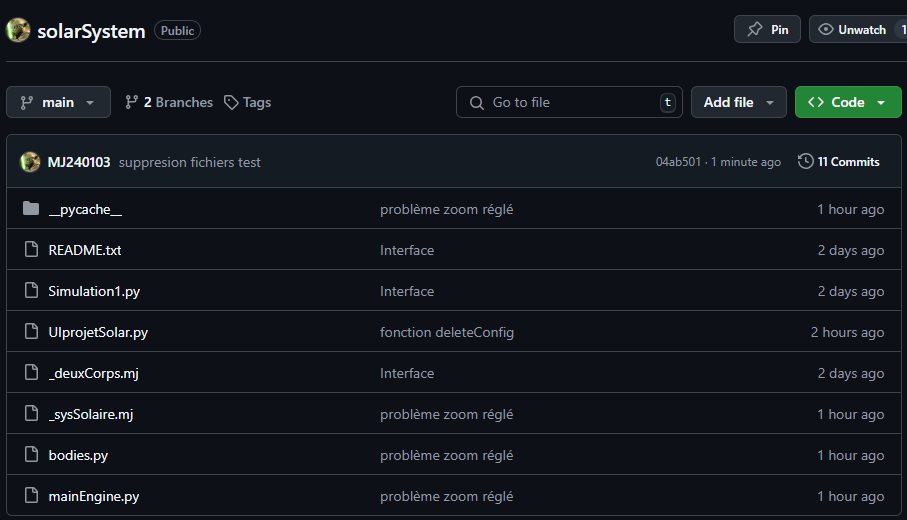
\includegraphics[width=0.5\linewidth]{imgGitHub.png}
        \caption{\label{fig:Git}Fichiers de la branche main du repository solarSystem.}
    \end{figure}

    \\

    Le fichier mainEngine.py utilise les équations et paramètres physiques du fichier bodies.py afin de simuler intéractions attractives entre un certain nombre de corps et avec certains paramètres par le biais de PyGame. Ce nombre de corps et ces paramètres seront définis par l'utilisateur grâce à l'application contenue dans le fichier IUsolarSystem. Celui-ci utilise Tkinter pour lancer la simulation PyGame. Les simulations peuvent être stockées dans des fichiers python (ex : Simulation1.py) ou dans des fichiers json (ex : sysSolaire.mj).

\section{Partie physique}
    \subsection{Implémentation naïve}

    \subsection{Implémentation avec Runge-Kutta d'ordre 4}

\section{Partie interface}
    \subsection{Interface de simulation avec pygame}

    \subsection{Intrface de l'application avec Tkinter}

\section{Exemples d'application}
    \subsection{Cas à deux corps}

    \subsection{Cas du système solaire}

\section{Conclusion et ouverture}


\end{document}